\chapter{Pruebas y Resultados}

A continuación se describirán las pruebas y resultados de trabajos similares, además de mostrar la planificación de pruebas para el presente trabajo.


\section{Pruebas y resultados en trabajos similares}

En \cite{mnih2015human} se usan como métricas el score promedio por episodio y el valor de acción promedio (Figura \ref{fig:dqn_results}). Luego se compara la eficiencia del agente de \ac{RL} con un jugador humano experto, siendo que el jugador humano tiene un 100\% de eficiencia, el agente de \ac{DQN} logra más de 100\% de eficiencia en 29 juegos de un total de 49 (Figura \ref{fig:dqn_vs_human}).

\begin{figure}[htb]
\centering
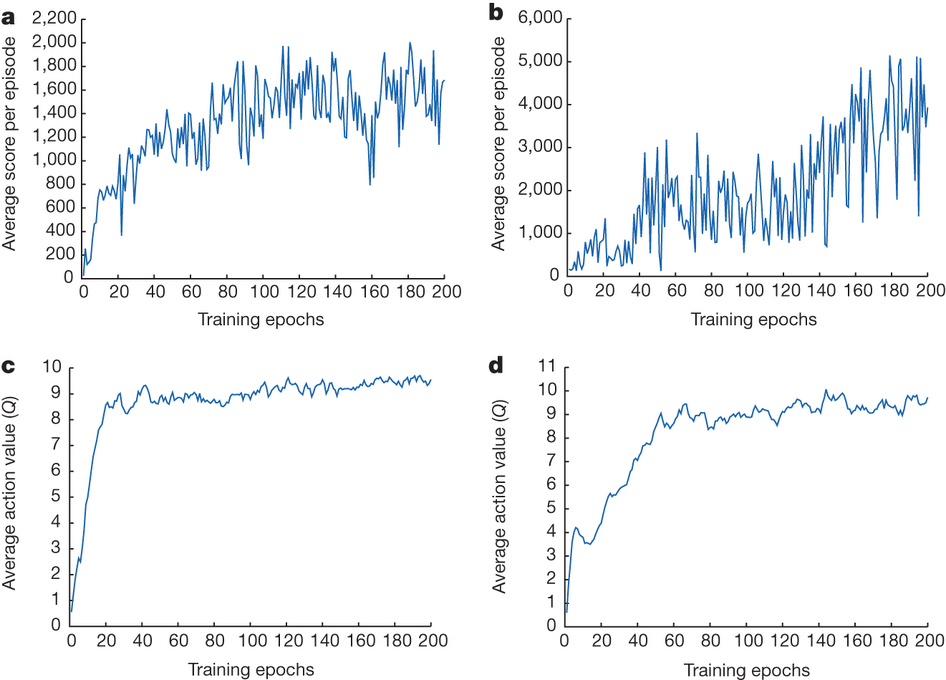
\includegraphics[width=150mm]{./graficos/dqn_results.jpg}
\caption{Resultados con DQN} \label{fig:dqn_results}
\end{figure}

\begin{figure}[htb]
\centering
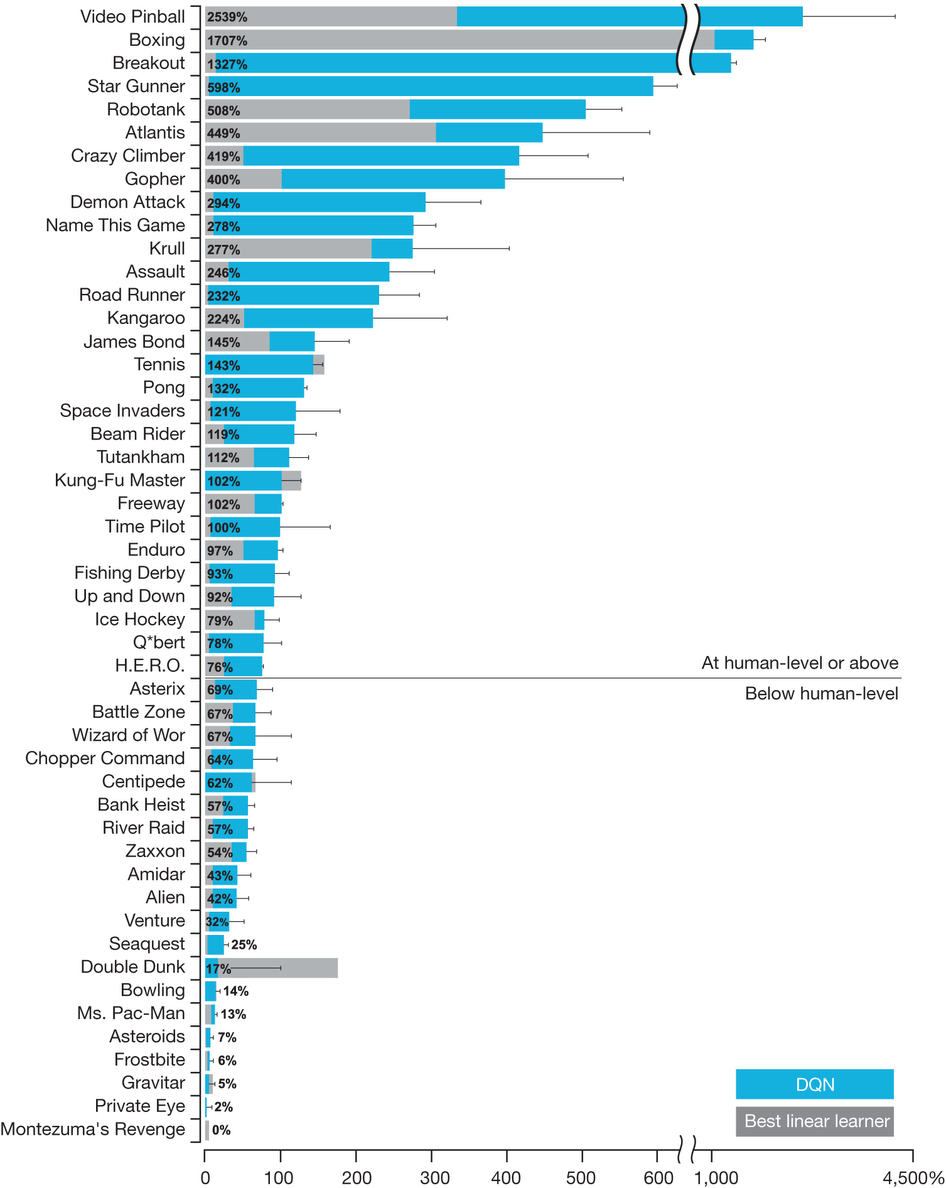
\includegraphics[width=150mm]{./graficos/dqn_vs_human.jpg}
\caption{DQN vs humano experto} \label{fig:dqn_vs_human}
\end{figure}

En \cite{silver2014deterministic} se usa una versión continua del problema de los bandidos para hacer una comparación directa entre las gradientes de política estocástica y deterministica. Luego se usan problemas donde el espacio de acciones es continuo y se comparan varios algoritmos recientes de \ac{RL} usando como métrica la recompensa total por episodio (Figura \ref{fig:dpg_results}).

\begin{figure}[htb]
\centering
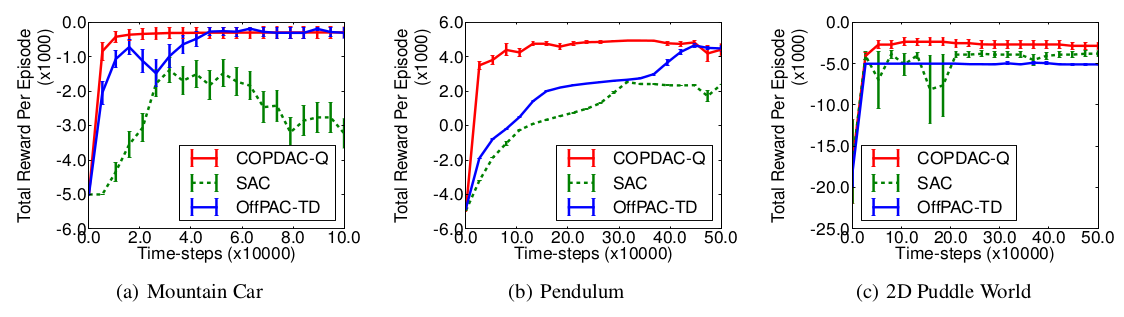
\includegraphics[width=150mm]{./graficos/dpg_results.png}
\caption{Resultados de \ac{DPG}} \label{fig:dpg_results}
\end{figure}

En \cite{lillicrap2015continuous} se utilizaron ambientes físicos simulados de varios niveles de dificultad para probar el algoritmo. Esto incluyo ambientes clásicos de \ac{RL} como cartpole, así como también tareas difíciles de alta dimensionalidad como brazos manipuladores o locomoción de esqueletos. Para la comparación se usa la recompensa normalizada (Figura \ref{fig:modified_dpg_results}).

\begin{figure}[htb]
\centering
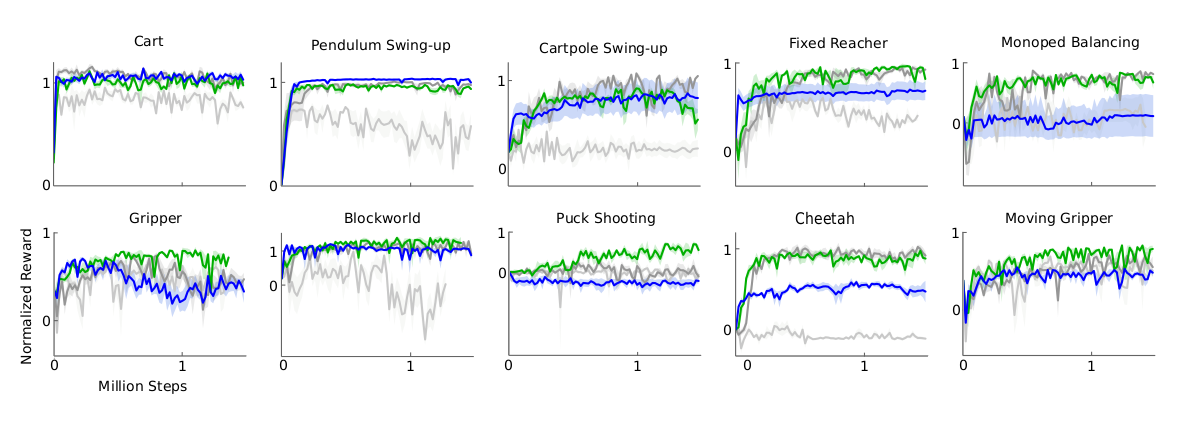
\includegraphics[width=150mm]{./graficos/modified_dpg_results.png}
\caption{Resultados de \ac{DPG} modificado} \label{fig:modified_dpg_results}
\end{figure}

\section{Planificación de pruebas}

Durante el entrenamiento del equipo se pretende registrar la recompensa por episodio, para evaluar la velocidad de convergencia.

Una vez que el equipo esté listo, se jugarán 50 partidos contra agent2D, registrando partidos ganados, perdidos y cantidad de goles. Si el número de partidos ganados es superior al 60\%, diremos que alcanzamos el objetivo.